%%%%%%%%%%%%%%%%%%%%%%%%%%%%%%%%%%%%%%%%%%%%%%%%%%%%%%%%%%%%%%%%%%%%%%%%%%%%%%%%
%2345678901234567890123456789012345678901234567890123456789012345678901234567890
%        1         2         3         4         5         6         7         8

\documentclass[letterpaper, 10 pt, conference]{ieeeconf}  % Comment this line out if you need a4paper

%\documentclass[a4paper, 10pt, conference]{ieeeconf}      % Use this line for a4 paper

\IEEEoverridecommandlockouts                              % This command is only needed if 
                                                          % you want to use the \thanks command

\newcommand{\ub}{\bar{u}}
\newcommand{\yb}{\bar{y}}
\newcommand{\wb}{\bar{w}}
\newcommand{\Hc}{\mathcal{H}}
\newcommand{\figref}[1]{Fig.~\ref{fig:#1}}
\overrideIEEEmargins       
\usepackage{todonotes}                              
\RequirePackage{graphicx}
\graphicspath{ {figures/} }
\usepackage[tight,footnotesize]{subfigure}

% See the \addtolength command later in the file to balance the column lengths
% on the last page of the document

% The following packages can be found on http:\\www.ctan.org
%\usepackage{graphics} % for pdf, bitmapped graphics files
%\usepackage{epsfig} % for postscript graphics files
%\usepackage{mathptmx} % assumes new font selection scheme installed
%\usepackage{times} % assumes new font selection scheme installed
%\usepackage{amsmath} % assumes amsmath package installed
%\usepackage{amssymb}  % assumes amsmath package installed

\title{\LARGE \bf
Requirements-Guided Closed-Loop Testing of Cardiac Devices
}

\author{Houssam Abbas and  Zhihao Jiang and Rahul Mangharam$^{1}$% <-this % stops a space
\thanks{*This work was partially supported by the grants NSF CAREER 1253842 and NSF MRI 566112.}% <-this % stops a space
\thanks{$^{1}$The Department of Electrical and Systems Engineering, University of Pennsylvania, Philadelphia, U.S.A.
        {\tt\small \{habbas,zhihaoj,rahulm\}@seas.upenn.edu}}%
}


\begin{document}

\maketitle
\thispagestyle{empty}
\pagestyle{empty}


%%%%%%%%%%%%%%%%%%%%%%%%%%%%%%%%%%%%%%%%%%%%%%%%%%%%%%%%%%%%%%%%%%%%%%%%%%%%%%%%
\begin{abstract}
Ventricular Fibrillation is a disorganized electrical excitation of the heart that results in inadequate blood flow to the body.
It usually ends in death within seconds.
The most common way to treat the symptoms of fibrillation is to implant a medical device, known as an \emph{Implantable Cardioverter Defibrillator} (ICD), in the patient's body.
Model-based verification can supply rigorous proofs of safety and efficacy. 
In this paper, we build a hybrid system model of the human heart+ICD closed loop, and show it to be a \yhl{STORMED system, a class of o-minimal hybrid systems that admit finite bisimulations.}
In general, it may not be possible to compute the bisimulation.
We show that approximate reachability can yield a finite \emph{simulation} for STORMED systems, which improves on the existing verification procedure.
In the process, we show that certain compositions respect the STORMED property.
Thus it is possible to model check important formal properties of ICDs in a closed loop with the heart, such as delayed therapy, missed therapy, or inappropriately administered therapy. 
The results of this paper are theoretical \yhl{and motivate the creation of concrete model checking procedures for STORMED systems.}
\end{abstract}

%Ventricular Fibrillation is a disorganized electrical excitation of the heart that results in inadequate blood flow to the body.
%It usually ends in death within a few seconds.
%The most common way to treat the symptoms of fibrillation is to implant a medical device, known as an Implantable Cardioverter Defibrillator (ICD), in the patient's body.
%Model-based verification can play a crucial role in ICD development.
%In this paper, we build a hybrid system model of the human heart+ICD closed-loop system, and show that it admits a finite bisimulation by showing it to be a STORMED hybrid system.
%In general, it may not be possible to compute the bisimulation.
%We show that approximate reachability can yield a finite \emph{simulation} for STORMED systems, which improves on the existing verification procedure.
%In the process, we show that certain compositions respect the STORMED property.
%Thus it is possible to model check important formal properties of ICDs in a closed loop with the heart, such as delayed therapy, missed therapy, or inappropriately administered therapy. 
%The results of this paper are theoretical, since no model checkers exist for STORMED systems. 
%In future work we will implement a procedure for model checking the heart+ICD loop.
\section{Introduction}
\label{introduction}

%\todo[inline]{stress the timing aspect more}
Implantable medical devices such as pacemakers are designed to improve physiological conditions with very little human intervention. 
Their ability to autonomously affect the physiological state of the patient makes the medical devices safety-critical, and sufficient evidence for their safety and efficacy should be provided before the devices can be implanted in the patients. Medical devices increasingly rely on software, and device function and their clinical performance can be affected by seemingly minor changes to software.
%As more functionality is added to the devices
\footnote{In what follows, the word `device' is used to refer to the software of the device.}
%, the complexity of the software component of the device is increasing dramatically, leading to a large number of potential safety violations because of software bugs. 

Over the course of the past four decades, cardiac rhythm management devices such as pacemakers and implantable cardioverter defibrillators (ICD) have grown in complexity and now have more than 80,000 to 100,000 lines of software code~\cite{pauljones}. In 1996, 10\% of \emph{all} medical device recalls were caused by software-related issues and this rose to 15\% between 2003-2012~\cite{recall_stats,killedbycode}. There is currently no standard for testing, validating, and verifying the software for implantable medical devices~\cite{fda1,fda3}.

There are two categories of device bugs: 
1) the device may fail to conform to its \emph{specifications}, that is, the prescription of how it should react to certain inputs.  
2) the device may fail to improve the conditions of the patient as promised, even if it conforms to its specifications. 
The desired physiological conditions that the closed-loop system should achieve are captured in the \emph{physiological requirements}; for example, for a pacemaker, the heart rate should always be maintained above a certain threshold. 
%In what follows, the word `requirement' always refers to such physiological requirements.
%Note that requirements are about \emph{the closed-loop system}: they prescribe the behavior of both device and environment (e.g. both pacemaker and heart).

Bugs in the first category (non-conformance to specification) can be detected via systematic and extensive open-loop testing in which a set of input sequences is fed to the device, and its output is compared with the expected output.
Bugs in the second category (violation of physiological requirements), on the other hand, require the availability of the \emph{closed-loop system}, which consists of the device and its environment.
For instance, the pacemaker and the heart as its environment. 
In the medical device industry, closed-loop verification of the physiological requirements is mostly performed in terms of clinical trials, in which the actual devices are implanted in human subjects over an extended duration.
Unfortunately, because of the extremely high cost of clinical trials (several million dollars and spanning several years~\cite{trial_cost}), the amount and variety of human subjects during the clinical trials are limited, which reduces the opportunity to find bugs. 
Moreover, clinical trials are often conducted at the final design stage. Fixing bugs at this stage is very costly.

Closed-loop model checking enables closed-loop evaluation of the physiological requirements at an earlier design stage, which requires formal model(s) of the physiological environment. 
%Depending on the formalism used to model the environment (and device) and the language used to express the requirements, this allows the usage of formal methods to perform the verification.
%Formal environment modeling introduces new challenges that do not arise when modeling the device alone, and this paper aims at addressing these issues in the context of pacemaker verification.
%In the rest of this paper, we speak therefore of pacemaker as the Device Under Verification (DUV) and of the heart as being the environment, but it is understood that the discussion carries more broadly, with possible domain-specific adjustments.
In closed-loop model checking, there is only one device model. 
However there can be a large number of environmental conditions which require different models to represent them. For instance, a heart with atrial flutter has an additional conduction pathway that is not present in a healthy heart, causing fast atrial rate. The timing and structural differences of different heart conditions should be distinguished in corresponding heart models.
%\todo[inline]{should we give an example of a heart condition?}
A set of initial models of the environment can be constructed but the set is inherently incomplete because of the large number of environment conditions and their combinations. 
As a result, performing model checking using every model in the set cannot ensure full coverage of the environmental conditions. 

In this paper, domain-specific over-approximation rules are developed that produce abstract models that not only cover explicitly modeled environment conditions, but also cover timing behaviors and conditions not modeled in the set of initial models. 
The abstract models can be then used for closed-loop model checking of the device model. 
If the closed-loop system satisfies a requirement, the device under verification satisfies the requirement under environment conditions covered by the abstract models. 
However, if the requirement is not satisfied, the model checker returns a counter-example. 
In device modeling, the counter-example is considered \emph{spurious} if it can not be produced by the device (as shown in (\figref{distinction}(a)).
However in environment modeling, even if the counter-example can not be produced by any of the initial environment models, it might still be a physiologically valid behavior.
Thus the validity of a counter-example cannot be determined by refining the environment model, but can ultimately only be determined by domain experts. 

Counter-examples returned from abstract models can be difficult to interpret by domain experts.
One abstract counter-example could be produced by multiple physiologically valid conditions, which causes ambiguity.
Thus, a rigorous framework is necessary to balance the need to cover a wide range of environmental conditions and the need to provide counter-examples to the physicians within their physiological context.

Another challenge for closed-loop model checking of medical devices is the amount of domain expertise needed during: 1) physiological modeling, 2) model abstraction and refinement, and 3) checking the validity of counter-examples.
Thus the framework must also allow non-domain experts to perform verification (item 2 above),
and establish `hand-off' points where the results of verification can be handed back 
to the experts for interpretation.

\begin{figure}[!t]
		\centering
		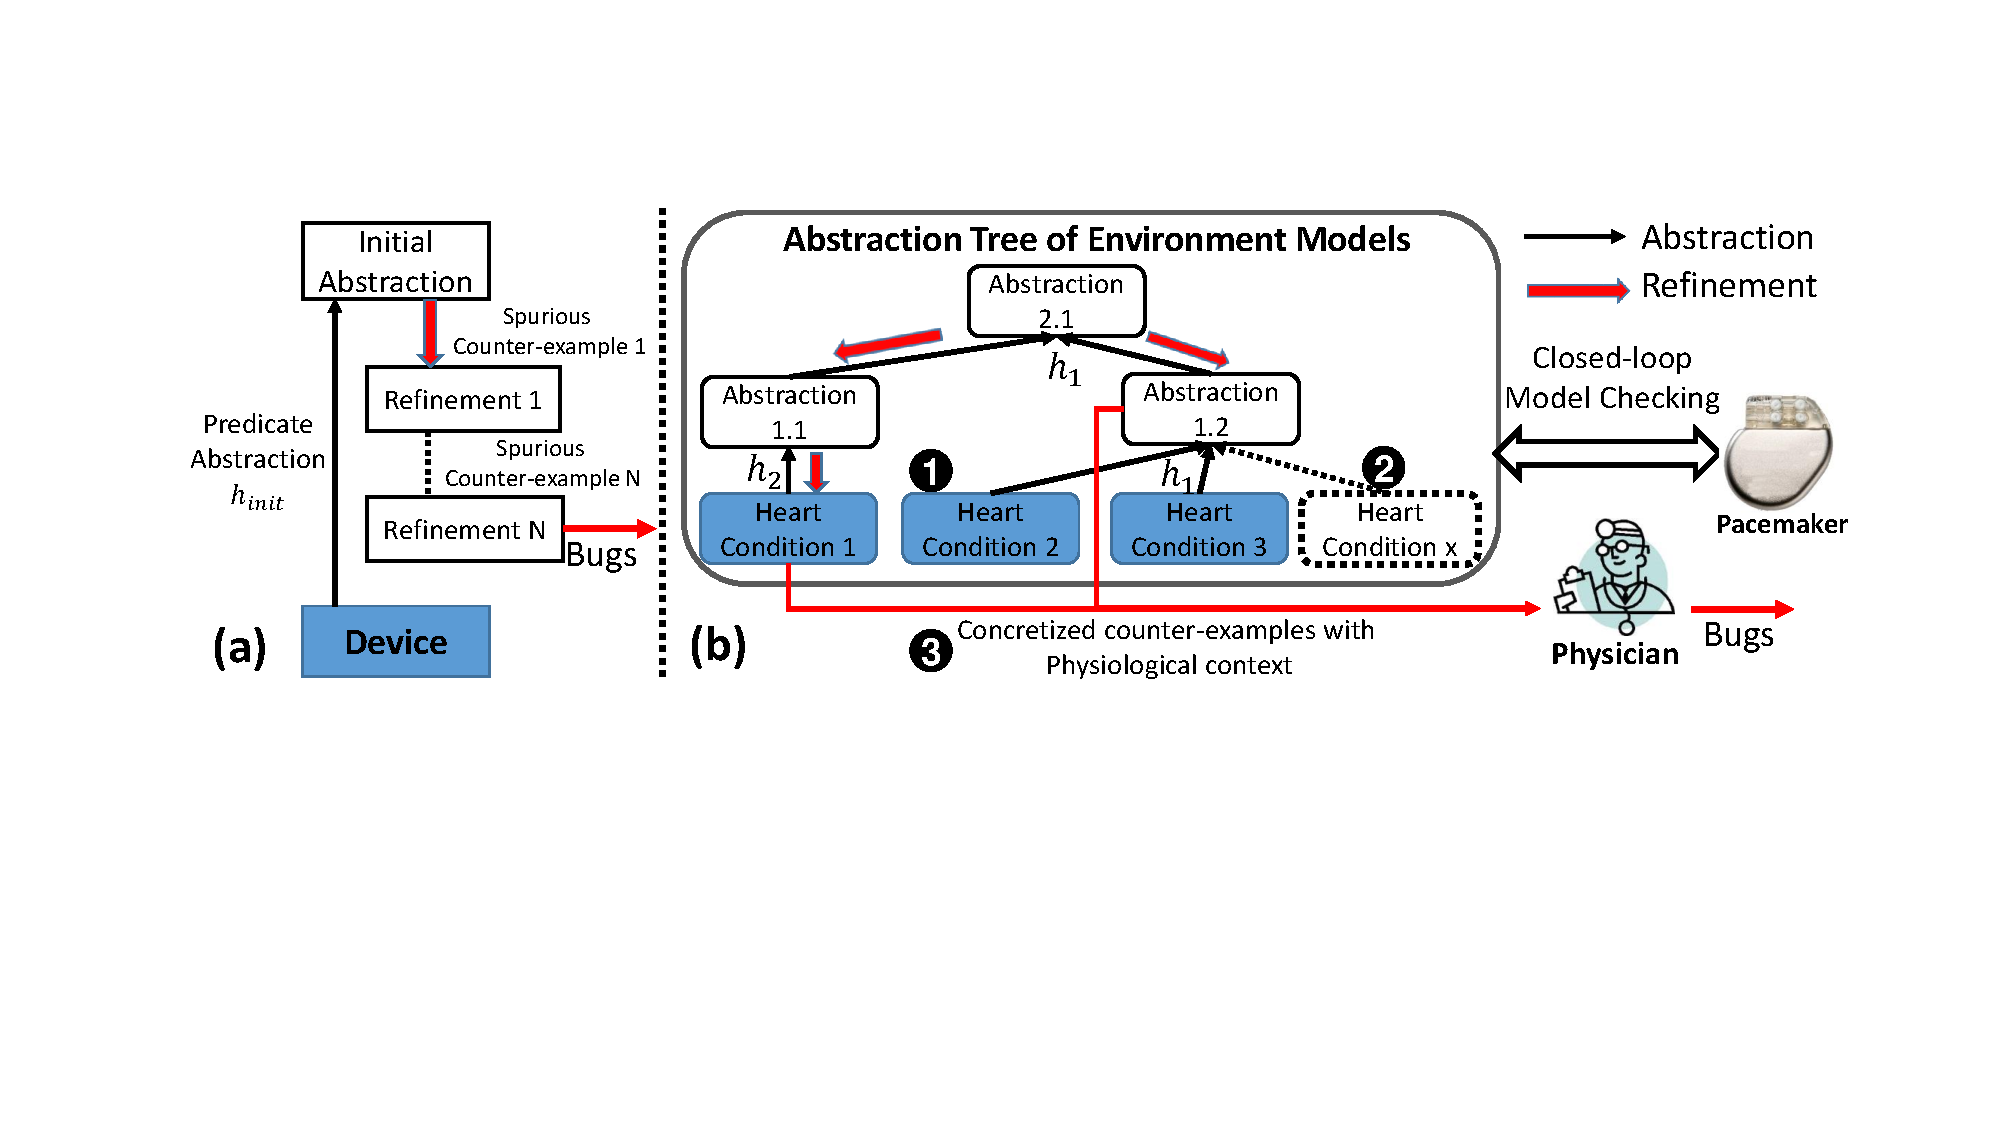
\includegraphics[width=\textwidth]{figs/distinction.pdf}
		%\vspace{-5pt}
		\caption{\small (a) Device modeling with CEGAR framework (b) Closed-loop model checking with environment abstraction tree.}% The initial set of heart conditions are first abstracted and/or merged using abstraction rules $h_1,h_2$ (Marker 1). The abstract model is first used for closed-loop model checking. When a property violation happens, refined models in the abstraction tree are used for model checking. The most concrete counter-examples may be available in the initial model(s) (Marker 2). In the scenario where counter-examples do not exist in explicitly modeled Heart condition 2 and 3, the counter-example in Abstraction 1.2 may correspond to a valid heart condition introduced during abstraction $h_1$. The physician decides the validity of the counter-examples.}
		  \vspace{-10pt}
		\label{fig:distinction}
\end{figure}


\subsection{Contributions}
In this paper a framework is proposed for environment modeling in closed-loop model checking of medical device software.
The cardiac pacemaker is used as an example of applying this framework.
An expandable set of timed-automata heart models are first developed to represent different physiological conditions (\figref{distinction} Marker 1).
A set of domain-specific abstraction rules are then developed based on physiological knowledge, which help ensure the physiological relevance of the behaviors introduced into the abstract models (\figref{distinction} Marker 2).
Then the rules are applied to the initial set of physiological models to obtain an abstraction tree, which will be used for closed-loop model checking of the pacemaker. 
A straightforward search procedure is then used to conduct model checking using suitable heart models and return the most concrete and unambiguous counter-examples to the physicians for analysis (\figref{distinction} Marker 3).
In this framework, physiological knowledge is only needed when constructing the initial model set and when analyzing counter-examples. 
The application of the physiological abstraction rules and the verification procedure can be automated.
The proposed method can potentially be generalized to other domains in which the device operates in a large variety of environmental conditions.
\subsection{Related Work}
%\todo[inline]{complete}
Counter-Example Guided Abstraction Refinement (CEGAR) \cite{CEGAR} has been proposed to over-approximate the behaviors of the device using predicate abstraction (\figref{distinction}.(a)).
%Upon property violation the abstract counter-example is checked for its validity on the actual system. If the counter-example is \emph{spurious} the model is then refined to eliminate the spurious counter-example. 
%This process is then continued on the refined model until either a valid counter-example returns or no counter-examples are returned. 
CEGAR works well during device modeling, however, it cannot be applied to environment modeling for two reasons: 1)~predicate abstraction does not guarantee the validity of behaviors introduced into the model. In fact, for device modeling, all additional behaviors introduced into the abstract model are spurious. 2)~the validity of a counter-example cannot be checked automatically as in device modeling. 

Proof-based approaches have also been applied to verify  abstractions and refinements of pacemaker specification using Event-B~\cite{eventb}. However, the authors did not take into account environment behaviors thus the framework cannot be used for verifying physiological requirements.  

Physiological modeling of cardiac activities has been studied at various levels for different applications. In \cite{natalia}, the electrical activity of the heart is modeled with high spatial fidelity to study the mechanisms of cardiac arrhythmia. In \cite{radu}, formal abstractions of cardiac tissue have been studied to reduce the complexity of the heart tissue model. However, these two models do not focus on the interaction with the pacemaker, therefore cannot be used for closed-loop model checking. In \cite{marta}, hybrid automata models of the heart has been used to capture the complex beat-to-beat dynamics of the heart tissue. However the model cannot be used to cover behaviors across different heart conditions.

In previous work \cite{sttt13} a set of formal heart models covering various heart conditions at different abstraction levels was developed, and closed-loop model checking was performed on models of implantable pacemakers. 
However, the physiological knowledge required during each step of closed-loop model checking prevents the method to be practical.


%During the closed-loop model checking, the most abstract model(s) that are appropriate to the requirement are automatically selected as the initial environment models. If the requirement is satisfied, the system is safe under the environment conditions covered by the initial environment models. If the requirement is violated in certain initial environment model, the children of the model in the abstraction tree are used for model checking until 1) the leaves of the tree is reached, or 2) there is no violations in the child nodes. The counter-examples obtained at the most refined models are returned to the physician for validity check. This process is automated so that no domain knowledge is required for the person who performs model checking. It also ensures the most concrete counter-examples with unambiguous physiological context are returned to the physician for analysis. 
%The first challenge in closed-loop model checking of pacemakers is that the human heart displays a large number of different conditions, henceforth referred to as `physiological conditions'.
%E.g., one heart may display \emph{atrial fibrillation} where the upper chambers of the heart (the atria) produce an exceedingly fast beat that prevents proper blood pumping.
%Another heart may display Premature Ventricular Contraction (PVC) where a location in the ventricles produces electrical impulses at erratic time instants.\Hao{I don't think these two conditions make sense to the reader}
%Each such condition will require its own formal model, and some models may display more than one condition.
%In this paper, we build such a set of formal heart models using the timed automata formalism in Section ???.
%Performing model checking with each model separately, we seek a method that can combine models, and perform model checking on the merged model. 
%The combination of models must be such that if the merged model is correct (according to the requirements) then so is every model that was combined into it.
%We present \emph{abstraction rules} in Section ?? which allow us to do precisely that.

%This initial set of models will necessarily be \emph{incomplete} because the number of physiological conditions is too large, and some of the conditions are too ill-understood for modeling.
%Thus, unlike system modeling in which one typically starts from one ground truth model to be verified, our starting point is an \emph{incomplete set of environment models}.
%Because of this incompleteness, we seek abstraction rules that introduce new \emph{physiologically meaningful} behavior which might actually be produced by heart models not in the initial set.
%These then correspond to heart conditions not taken explicitly into account. 
%This provides a second motivation for the domain-specific abstraction rules $R$ in Section ???, which can be thought of as relaxations of the conditions governing the model's behavior. 
%Like predicate abstraction, they produce models that over-approximate the behavior of the model they are applied to (i.e., $\beh(R(M)) \supset \beh(M)$).
%However, the new behavior they introduce might not be spurious. 
%We demonstrate such a case in Section ???.
%If model checking returns a counter-example on $R(M)$, the physician can decide whether this is actually physiologically plausible behavior and therefore the pacemaker needs to be debugged, or this is indeed spurious and should be thrown out (and the abstraction refined).
%
%Note this is different from classical predicate abstraction [???], which adds behavior in a domain-agnostic fashion. In fact, predicate abstraction is a fist step in the timed automata model checking procedure as presented in [ALur and Dill 1994].
%Our abstraction rules are used to combine and and abstract models \emph{prior} to model checking.
%%tttt
%
%\subsubsection{Contributions}
%In this paper we propose a framework for environment modeling and model checking of medical device software, in particular, pacemakers.
%Specifically, we present several extended timed automata models of various heart conditions in Section ???. 
%We define domain-specific abstraction rules for these models, and demonstrate how these can be applied to gradually add physiologically meaningful behavior in Section ???. 
%Using the models and the rules, we build an abstraction tree which serves to perform model checking of physiological requirements for the heart+pacemaker closed loop in Section ???.
%We illustrate the approach via case studies in Section ???, and conclude in Section ???
%

%

\section{Method: Requirements-guided closed-loop testing}
\label{method}

%\begin{figure}[!t]
%	\centering
%	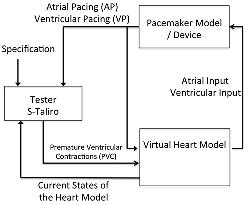
\includegraphics[scale=0.4]{reqGuidedTesting.pdf}
%	\caption{\small Requirements-guided closed-loop testing methodology.}
%	\label{fig:reqGuidedTesting}
%\end{figure} 
\begin{figure}[!t]
	\centering
	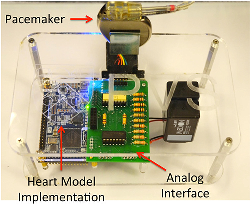
\includegraphics[scale=1.2]{figures/HOCannotated.pdf}		
	\caption{\small Heart-on-a-Chip platform, showing the pacemaker and the microcontroller running the Virtual Heart Model code.}
	\label{fig:hoc}
\end{figure} 

Figure \ref{fig:reqGuidedTesting} shows the requirements-guided closed-loop testing setup that we use in this paper to find unsafe or undesirable behavior of the heart connected to the pacemaker.
In what follows, we describe each component in details.

\input{heartModel}
\subsection{The Heart-on-a-Chip platform}
\label{HoC}

\begin{figure}[!t]
	\centering
	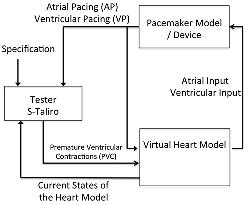
\includegraphics[scale=1.2]{reqGuidedTesting.pdf}
	\caption{\small Requirements-guided closed-loop testing methodology.}
	\label{fig:reqGuidedTesting}
\end{figure} 
%\begin{figure}[!t]
%	\centering
%	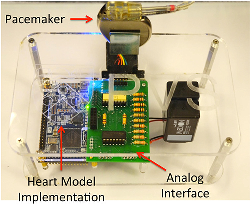
\includegraphics[scale=0.3]{figures/HOCannotated.pdf}		
%	\caption{\small Heart-on-a-Chip platform, showing the pacemaker and the microcontroller running the VHM code.}
%	\label{fig:hoc}
%\end{figure} 
Our closed-loop testing scheme can be performed not only on pacemaker models and code, but also on off-the-shelf pacemaker devices. 
\figref{hoc} shows the Heart-on-a-Chip (HoC) platform for closed-loop testing of pacemakers. 
The platform consists of a micro-controller running the code of the VHM, and an analog interface to the pacemaker. 
The analog interface converts VHM outputs to physiological heart signals, which will be input to the pacemaker, and converts pacemaker pacing signals to node activation events.  
A user interface on the host computer monitors the closed-loop interaction between the heart and the pacemaker and violations to the physiological requirements are reported.

\subsection{Closed-loop testing of pacemaker}
\label{closedloop}

\begin{figure}[t]
\centering
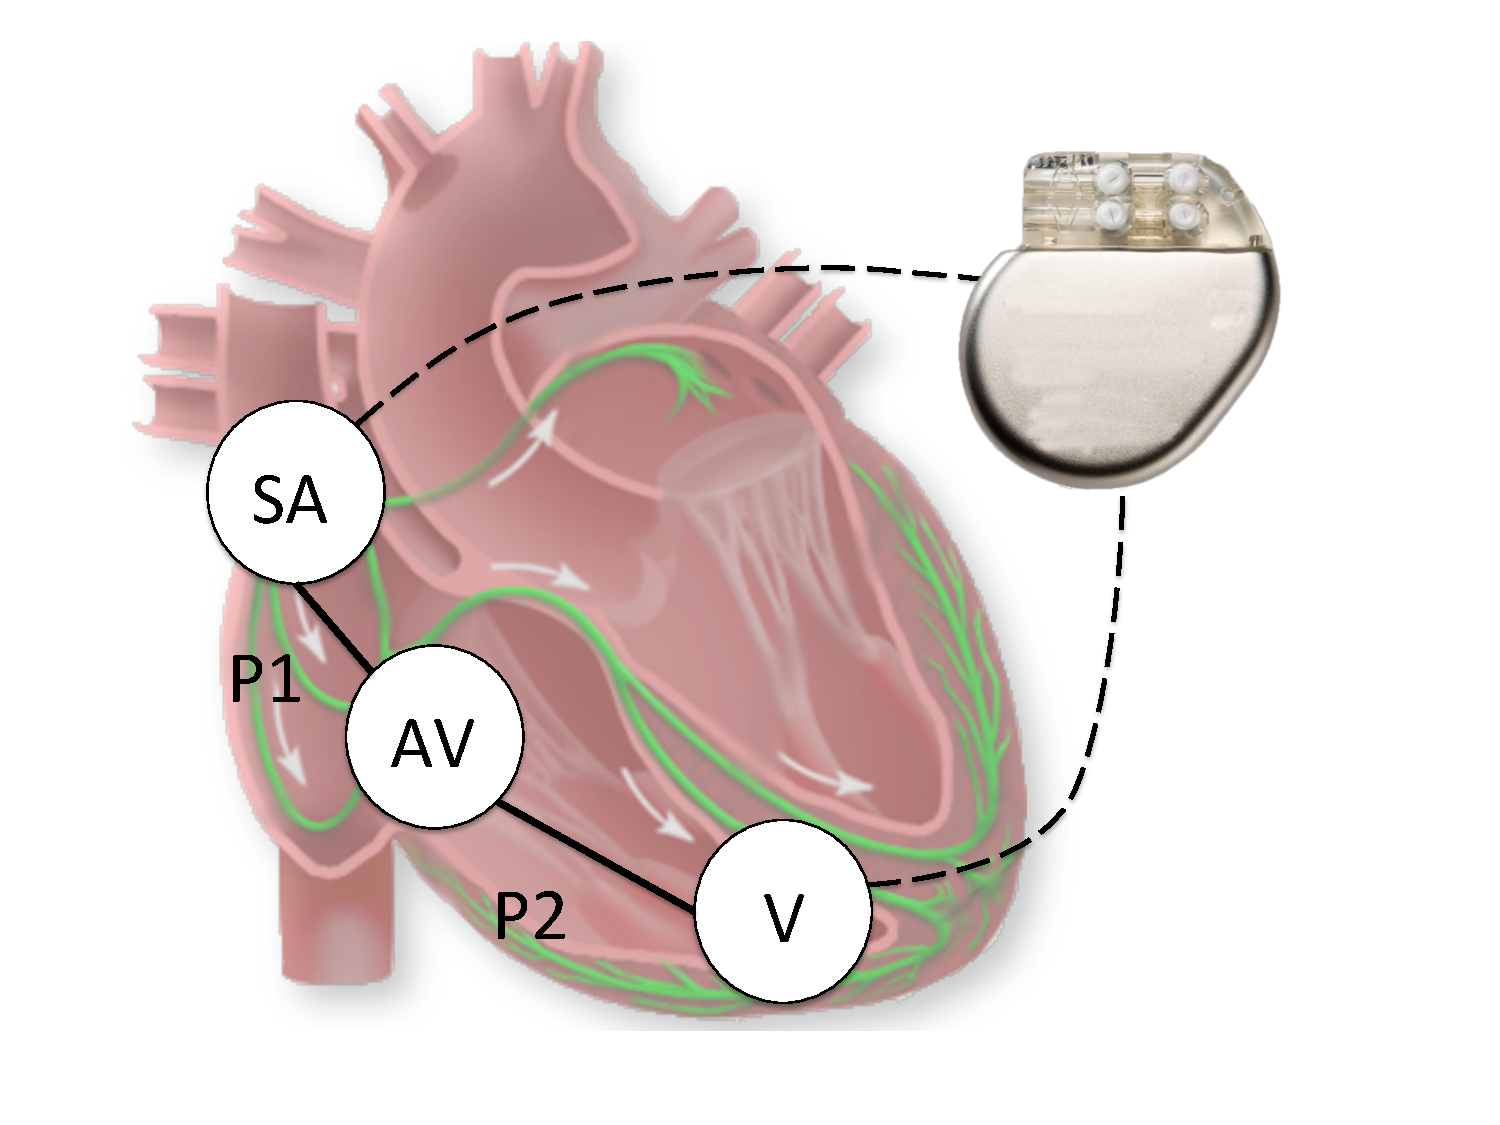
\includegraphics[scale=0.2]{figures/nodesandPM}
\caption{Portion of the VHM: the conduction paths P1 and P2 connect the SA node to the ventricle V via the AV node (solid line). The pacemaker induces a second, `virtual', pathway (dashed line).}
\label{fig:nodesandPM}
\vspace{-.5cm}
\end{figure}

\textbf{Closed-loop setup}.
The closed-loop setup is shown in Fig.~\ref{fig:reqGuidedTesting}.
The VHM and pacemaker are connected in the same way as a real heart and pacemaker would be connected.
Thus, the inputs to the pacemaker are automatically generated by the VHM as atrial and ventricular sensing events (AS and VS), and don't need to be pre-programmed by the validation engineer as they would be in open-loop testing. 
The VHM, in turn, is stimulated by the pacemaker's Atrial and Ventricular Pacing events (AP and VP).
In addition, the tester is connected at the PVC `inputs' to the heart.
That is, the tester provides waveforms that mimic PVC events as will be explained below.
The tester can read all required signals from the VHM.
In our experiments, it reads five waveforms: the depolarization events at SA node, AV node, and ventricle (SA, NA and V), and the conduction state of paths P1 and P2 connecting them. (See Fig.~\ref{fig:nodesandPM}.)
It also reads the AP and VP events from the pacemaker.

\textbf{Tester-controlled inputs}.
In our setup, the testing algorithm will generate Premature Ventricular Complex (PVC) waveforms to mimic the abnormal depolarizations of the ventricles that occur in the human heart, and can fool the pacemaker sensing. 
A \emph{test} is then defined as a PVC waveform of a pre-determined duration $T$ ms.
These are used by the tester to try and cause the closed loop to manifest unsafe or undesirable heart conditions.
The constraint on the waveforms generated by the tester is that there should be at least 400ms between consecutive PVC impulses.
More generally, the tester can also generate Premature Atrial Contraction (PAC) events and vary the closed loop parameters within their physiological range.

\textbf{The tester}.
The tester itself is a requirements-guided automatic test generation algorithm, whose theory is given in \cite{AbbasFSIG13tecs}, and we review it here briefly.
This testing algorithm has been implemented in the tool S-Taliro \cite{AnnapureddyLFS11tacas}, and has been used in other medical applications like the analysis of insulin infusion pumps schedules \cite{SankaranarayananF2012cmsb}.
The operation of the tester is as follows: we provide S-Taliro with a requirement that the pacemaker+heart closed loop must satisfy,
e.g., ``there should be a minimum delay of 500ms between VP events''.
S-Taliro performs an iterative optimization to find a test (i.e., a PVC waveform of pre-determined duration) such that the resulting closed loop behavior \emph{violates} the requirement.
The objective function of the optimization is directly related to the requirement, as detailed in \cite{AbbasFSIG13tecs}.
It can be shown that if the system can exhibit a behavior that violates the specification, then this process converges to a test that will provoke this incorrect behavior \cite{AbbasFSIG13tecs}. 
%This test then serves as evidence that the pacemaker+heart loop can exhibit undesired behavior that violates the specification.
The pacemaker's designer can then replay this test to see where things went wrong, and whether the pacemaker needs to be adjusted accordingly.

\textbf{Advantages over open-loop testing}.
The advantages of the proposed requirements-guided closed-loop testing approach over directed open-loop testing are summarized in Table \ref{table:CLoverOL}, and discussed here:
\begin{table*}
	\centering
	\caption{Comparison between open-loop and proposed closed-loop testing.}
	\begin{tabular}{|l|l|l|}
	\hline                       & Open-Loop    & Requirements-Guided Closed-Loop 
	\\ 
	\hline Choice of pacemaker input traces  
	                & Manual and recorded traces. Might miss interesting  &  Automatic and provided by the VHM,
	\\ 
					& behavior, or include irrelevant behavior. &  so only relevant input traces are used.
	\\
	\hline Criterion of correctness    & Only pacemaker behavior & The heart and pacemakers's joint behavior, so 
	\\
	                &                  & physiological effects of pacemaker actions
	\\
	                &                  &  can be used to determine correctness.                   
	\\ 
	\hline Choice of tests & Tests = input traces to pacemaker.  & Tests = traces of external disturbances, 
	\\
	                & Manually chosen.  & like PVC and PAC. Automatically selected by S-Taliro
	\\
	\hline 
\end{tabular}
\label{table:CLoverOL}
\end{table*}

\begin{figure}[t]
\centering
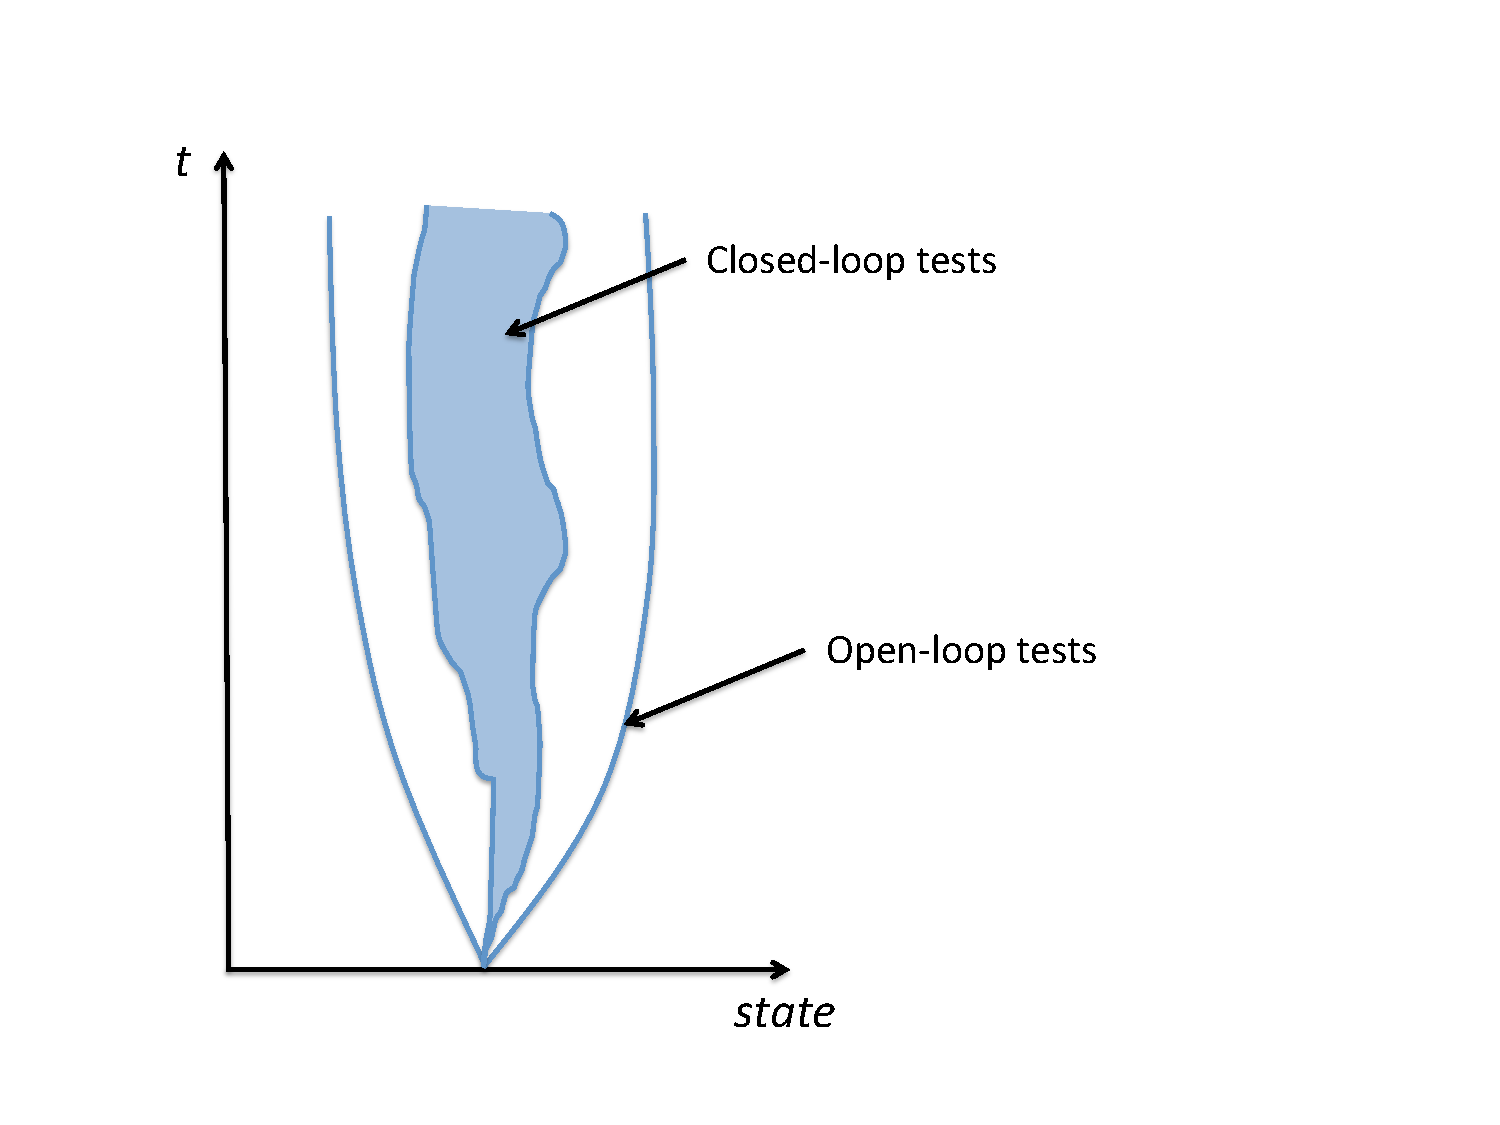
\includegraphics[scale=0.3]{figures/cone}
\caption{The space of closed-loop inputs to the pacemaker is constrained by the VHM and is thus smaller than the open-loop space.}
\label{fig:cone}
\vspace{-.2cm}
\end{figure}

\begin{itemize}
	\item Choice of inputs: because a heart model provides the input traces to the pacemaker, we know that only relevant test cases will be generated. 
	That is, only traces that the pacemaker may actually see during live operation are fed to it during testing. 
	\footnote{Of course, this ultimately depends on the quality of the VHM.}
	Compare this to open-loop testing where nothing constrains the inputs, as illustrated in Fig.~\ref{fig:cone}.
	It is difficult if not impossible to reason a priori about how the heart will constrain the pacemaker's inputs, especially for \emph{deep} behaviors that take a long time to occur.	
	Moreover, because the tester produces the tests systematically, we are guaranteed to find violating behavior if it exists.
	\item Criterion of correctness: because we have a VHM, we can express correctness \emph{as a property of the heart's behavior}, and not of the pacemaker alone. 
	Thus we can evaluate what truly matters: is the heart (as modeled by the VHM) displaying unsafe or undesirable behavior?
\end{itemize}

%\textbf{Choice of specifications to test}.
%Because the heart's behavior is complex and varies depending on its physiological structure and history, it is not always easy to describe succinctly what is `unsafe' and what is `undesirable'.
%Both categories vary depending on what we know (and what we discover) about the heart conditions being modeled.

\textbf{Interpretation of testing results}.
It must be stressed that the interpretation of closed-loop testing results depends on the specific violating behaviors that are found.
Some will be determined to be bugs in the pacemaker (or VHM). 
Others will be determined to be undesirable but unavoidable behaviors, and we show such a case in Section \ref{experiments}.
%This is because specifying `safe' behavior can be difficult for something as complex as the heart.



\section{Experiments}
\label{experiments}

%For the following two experiments, the pacemaker model is evaluated against two physiological requirements.
a) \emph{Exploring behavior}: In this experiment, we
%set a minimum delay of 400ms between PVC pulses, and 
tried to falsify the following specification:
``The interval between an activation of the ventricle node to a ventricular pacing (VP) should be longer than 500ms".
This specification is designed to identify closed-loop execution traces in which the pacemaker is pacing the heart too fast. %Note that the pacemaker can not distinguish between a VS caused by a PVC and a VS caused by path conduction.
%Thus we need access to the heart model to test this specification, and this can only happen in a closed-loop setting.

The specification was violated by the execution shown in Fig. \ref{fig:bug8_kept1}.
% This comes from bug8_kept1
\begin{figure}[tb]
\centering
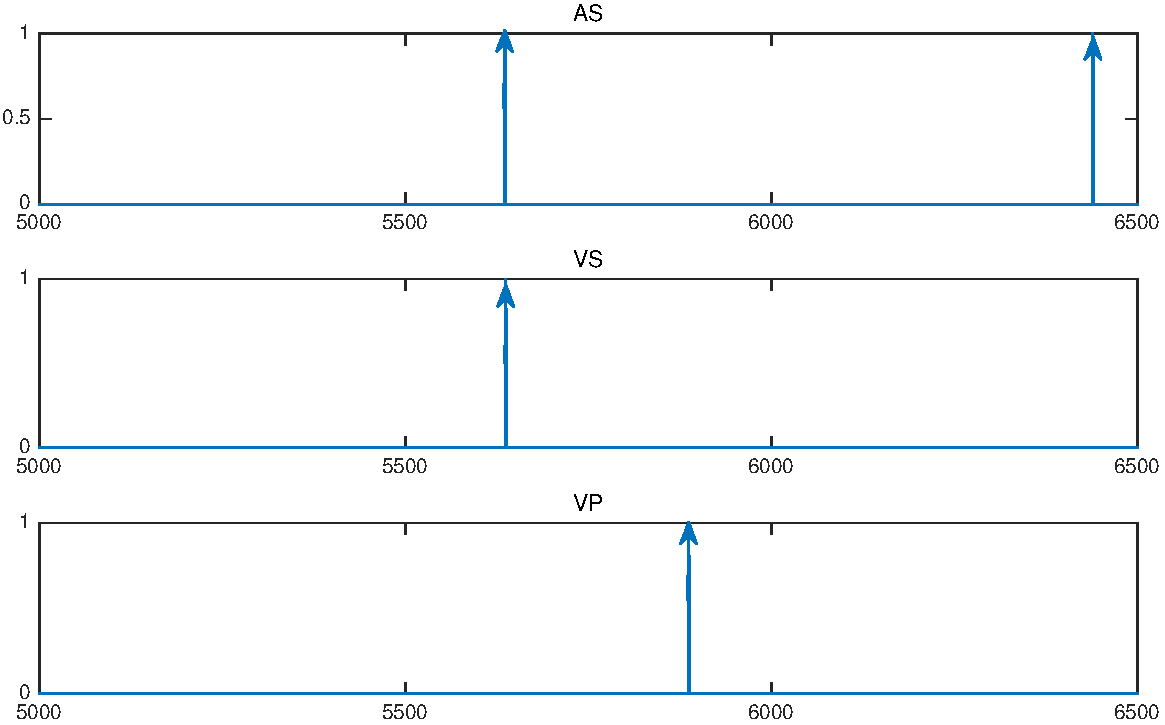
\includegraphics[width=0.7\linewidth]{figures/bug8_kept1}
\caption{A PVC pattern that causes a premature ventricular pacing.}
\label{fig:bug8_kept1}
\end{figure}
Upon investigating the reasons for this violation, it was concluded that one of the noise filters, the post-atrial ventricular blocking (PAVB) designed to avoid crosstalk between channels, caused the problem.  
A PVC happened shortly after an atrial sense (AS) which fell into the PAVB period and was ignored. 
Due to its limited sensing capability the pacemaker cannot distinguish noise from a valid input which happened at a rare time.
Thus, the designer and physician must decide whether this is an acceptable case, or the pacemaker needs to be adjusted (if at all possible) to prevent this from happening (while maintaining the VSP safety feature).

b) \emph{Finding harmful heart behavior}: In this experiment, we tested the closed loop to see if the pacemaker could lead the heart into a harmful condition known as Endless Loop Tachycardia (ELT).
%
The heart has one intrinsic conduction pathway from atria to ventricles, namely from the SA node to the ventricles via the AV node and His bundle.
The AVI period of the DDD pacemaker introduces another, virtual, pathway between the atrial lead and the ventricular lead.
See Fig.~\ref{fig:nodesandPM}.
%If a PVC happens shortly after a normal A-to-V conduction, the signal would go around the closed circuit formed by the heart and the pacemaker, inhibiting intrinsic heart signals and causing the heart to beat at a fixed high rate.
In an ELT, first, a PVC triggers V-A conduction along the intrinsic pathway, 
which in turn triggers an AS. 
The pacemaker will then pace the ventricle (issue a VP) after TAVI ms according to its A-V synchrony function. 
This VP then triggers another V-A conduction, and so on.
The conduction loop is then formed and the VP-AS pattern will persist if no actions are taken,
and the heart rate is kept as high as the upper rate limit of the pacemaker.% since the cycle length of the conduction loop is very short. 
As shown in Fig.\ref{fig:ambiguity}, the pacemaker's limited sensing capabilities can not distinguish between a PVC-induced VS and an intrinsic VS.
ELT is a harmful condition since a fast fixed heart rate that will cause inefficient pumping of blood.
Thus even though the pacemaker is correct according to its specification, it can still lead the heart into ELT if a PVC interferes with its operation as described.
%
\begin{figure}[t]
\centering
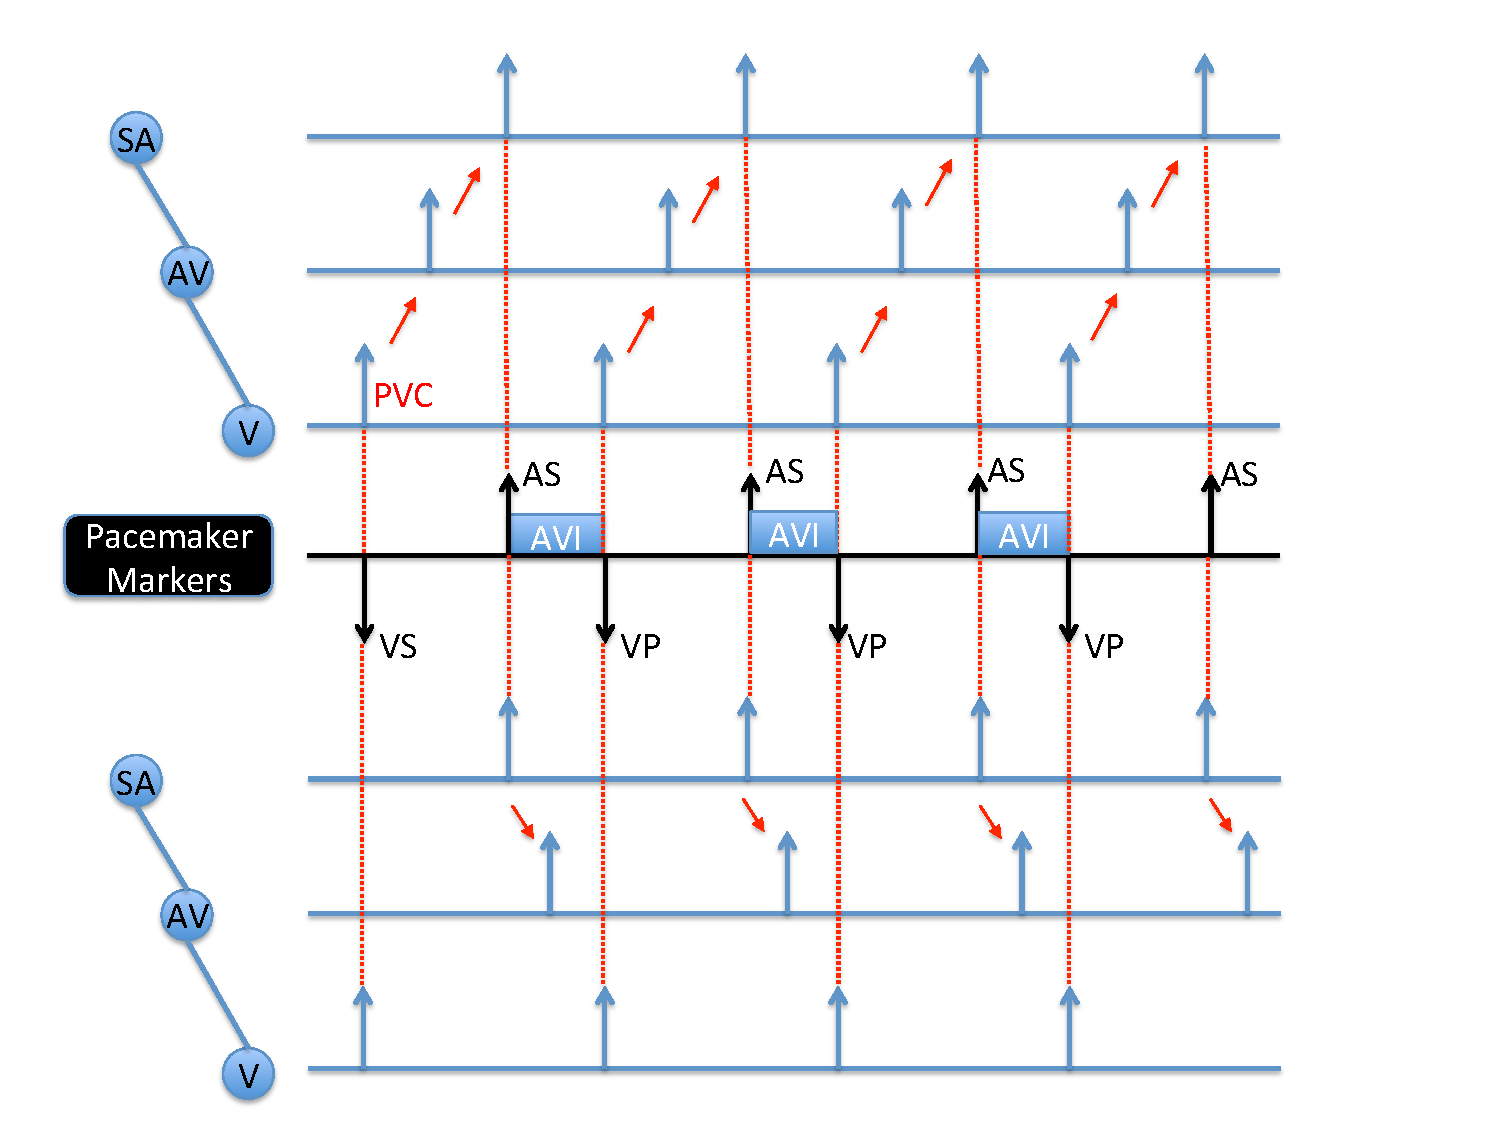
\includegraphics[scale=0.3]{figures/ambiguity}
\caption{An ELT sequence (above the Markers line) and an intrinsic conduction (below it) cause the same sensed events in the pacemaker.}
\label{fig:ambiguity}
\vspace{-0.7cm}
\end{figure}
S-Taliro was given the ELT specification, and a PVC constraint of at most 2 PVCs in a 10,000ms interval. 
The total test duration was $T= 10,000$ms.
S-Taliro found a PVC pattern, shown in Fig.~\ref{fig:bug13_kept1}, that caused ELT.
% This is bug13_kept1
\begin{figure}[t]
\centering
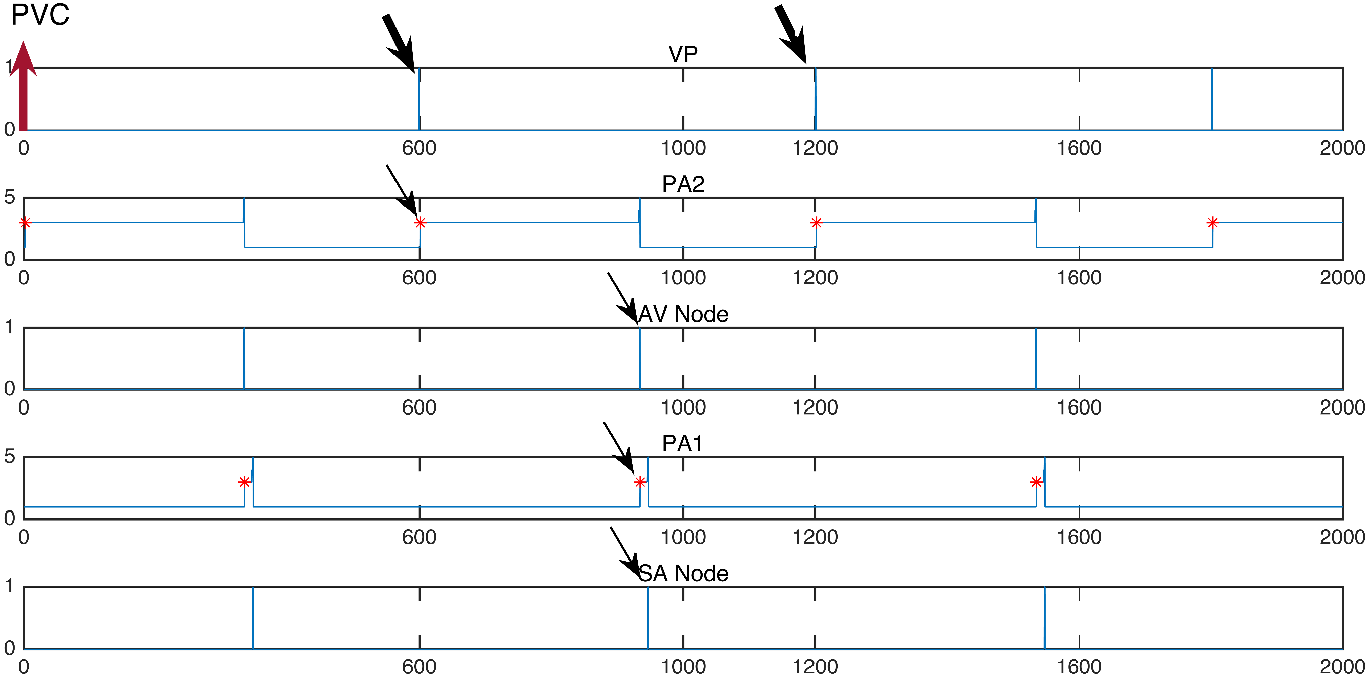
\includegraphics[height=0.2\textheight,width=1\columnwidth]{figures/markedELT.pdf}
\caption{ELT. The vertical red arrow indicates the initial PVC, thick arrows indicate the beginning of each ELT cycle, and thin arrows indicate the events involved in the ELT diagnosis.}
\label{fig:bug13_kept1}
\end{figure}



\section{Conclusion}
\label{sec:conclusion}

Clinical trials study the effect of an intervention \emph{in the patient}, and report patient-level results (e.g., ``The event of interest was observed in X\% of patients in Group 1''). 
Our results are at the condition level: they take the form ``the event of interest was observed in X\% of generated conditions".
To produce patient-level estimates requires an estimate of how conditions are distributed among patients. 
This low-level data is not publicly nor readily available.
A trial's investigators, however, should be able to obtain such data from previous trials.

It is important to stress that in general, one should not expect \emph{absolute numbers} from an MBCT to match those from a clinical trial, nor should this be the goal of the MBCT.
For example, in this work, it is unlikely that our MBCT will yield rates of inappropriate therapy that are equal to the rates obtained by RIGHT itself.
The reasons for this are many:
\begin{itemize}
	\item The RIGHT in vivo cohort, and our synthetic cohort, are not comparable:
	indeed, a myriad of factors affect the outcome of a clinical trial, e.g., whether some patients take up smoking. 
	These factors are not modeled.
	\item The adjudication of episodes in RIGHT (and other trials) is limited by the fact that only therapy episodes were recorded by the devices.
	The adjudication process is further limited by the lack of surface EKGs, which makes it hard to reliably distinguish certain atrial arrhythmias. 
	Neither of these is a limitation in MBCT since we have the ground truth: we know exactly what arrhythmia is being simulated by the model.  Furthermore, the AAEL signals have both device electrograms (EGMs) and the corresponding surface EKGs which allow for precise adjudication.  
	\item Experts may disagree on how to adjudicate the more complex episodes, so our classification of episodes from the AAEL database and the classification of the RIGHT investigators have an irreducible discrepancy.
	Again, this will affect the statistics that they and we compute.
\end{itemize}

That said, we can expect that a good heart model will reveal \emph{the trend} of the results, such as improvement of intervention over control or not, as shown in this paper. 
The MBCT conducted here clearly showed that the Medtronic algorithms outperforms the Boston Scientific's and resulted in a negative outcome of RIGHT across all population distributions and relevant heart conditions. In hindsight, the Boston Scientific-sponsored RIGHT would have needed reconsideration prior to running it to prevent a failed outcome.




\bibliographystyle{abbrv}
\bibliography{EMBC2015,conformance,conformanceMEMOCODE,fainekos_bibrefs}  




\end{document}
